% L5b student companion deck.
%
% The frame order mirrors the lecture notebook so students can take notes while
% the instructor works through the notebook. The disclaimer is intentionally
% slide 2, by instructor preference.
\documentclass[aspectratio=169,11pt]{beamer}
\usepackage{vnslides}

\newcommand{\Pmeasure}{\mathbb{P}}
\newcommand{\E}{\mathbb{E}}
\newcommand{\Var}{\operatorname{Var}}
\newcommand{\Cov}{\operatorname{Cov}}
\newcommand{\gbar}{\bar g}
\newcommand{\bA}{\mathbf{A}}
\newcommand{\bC}{\mathbf{C}}
\newcommand{\bG}{\mathbf{G}}
\newcommand{\bZ}{\mathbf{Z}}
\newcommand{\bw}{\mathbf{w}}
\newcommand{\bg}{\mathbf{g}}
\newcommand{\Sg}{\hat{\boldsymbol{\Sigma}}_{g}}
\newcommand{\Ch}{\hat{\mathbf{C}}}

\title{\texorpdfstring{{\vnheavy L5b}}{L5b}: Multiple Asset Geometric Brownian Motion}
\subtitle{CHEME 5660 Cornell University}
\author{Copyright Jeffrey Varner 2026. All Rights Reserved}

\begin{document}

\vntitlepage

\begin{frame}{Disclaimer and Risks}
  \vspace{0.6em}
  \textbf{\ink{Training only.}} This content is for training and informational
  purposes only. The teaching team does not make, give, or endorse any offer or
  solicitation to buy or sell securities or derivative products, or provide
  investment or trading advice or strategy.

  \vspace{1.1em}
  \textbf{\ink{Risk.}} Trading involves risk and is generally not recommended for
  those with limited resources, experience, or a low risk tolerance. Past
  performance does not guarantee future success.

  \vspace{1.1em}
  \textbf{\ink{Responsibility.}} You are responsible for your investment decisions
  based on your financial circumstances, objectives, risk tolerance, and
  liquidity needs.
\end{frame}

\begin{frame}{Objectives for Today}
By the end of this lecture, you will be able to:

  \vspace{0.8em}
  \begin{itemize}\setlength{\itemsep}{0.8em}
    \item \hilite{Update and extend GBM}: update single asset GBM parameters
      with an exponential moving average, then model several assets whose
      prices move together.
    \item \hilite{Estimate and interpret covariance}: calculate the covariance
      matrix from historical growth rates, interpret covariance and
      correlation, and convert it to the model's covariance rate.
    \item \hilite{Compare portfolio allocations}: relate weights to
      buy-and-hold wealth, generate long-only allocations with the Dirichlet
      distribution, and compare their estimated growth and risk.
  \end{itemize}
\end{frame}

\begin{frame}[t]{Lectures and Examples}
\small
\textbf{\ink{Lecture:}}
  \href{https://github.com/varnerlab/CHEME-5660-CourseRepository-Fall-2026/blob/main/lectures/week-5/L5b/CHEME-5660-L5b-Lecture-MultipleAsset-GBM-Fall-2026.ipynb}{Multiple Asset Geometric Brownian Motion}

  \vspace{0.4em}
  \textbf{\ink{Example:}}
  \href{https://github.com/varnerlab/CHEME-5660-CourseRepository-Fall-2026/blob/main/lectures/week-5/L5a/CHEME-5660-L5a-Example-EMA-SAGBM-Fall-2026.ipynb}{Updating GBM Parameters with EMA}

  Carried over from L5a. Can recent observations improve the forecasts? Update
  mean growth and volatility, then compare the forecasts with the frozen model.

  \vspace{0.4em}
  \textbf{\ink{Example:}}
  \href{https://github.com/varnerlab/CHEME-5660-CourseRepository-Fall-2026/blob/main/lectures/week-5/L5b/CHEME-5660-L5b-Example-CovarianceMatrix-Fall-2026.ipynb}{Covariance and Correlation from Data}

  How do firms' growth rates move together? We estimate covariance and
  correlation from historical data and connect them to the price model.

  \vspace{0.4em}
  \textbf{\ink{Example:}}
  \href{https://github.com/varnerlab/CHEME-5660-CourseRepository-Fall-2026/blob/main/lectures/week-5/L5b/CHEME-5660-L5b-Example-Dirichlet-PortfolioWeights-Fall-2026.ipynb}{Portfolio Weights and the Dirichlet Distribution}

  How does the investment mix affect growth and risk? We explore portfolio
  weights with the Dirichlet distribution and follow buy-and-hold wealth.
\end{frame}

\begin{frame}{Concept Review: Updating GBM Parameters}
An \hilite{exponential moving average (EMA)} updates the GBM estimates as
new prices arrive, giving recent growth rates $g_k=\ln(S_k/S_{k-1})/\Delta t$
more weight.

\vspace{0.5em}
Initialize at entry index $s$ from the training estimates:
\[
  m_s=\hat\mu_{g,0},\qquad v_s=\frac{\hat\sigma_0^2}{\Delta t}.
\]
With decay factor $0<\lambda<1$, update at each new observation $k>s$:
\[
\begin{aligned}
  \delta_k &= g_k-m_{k-1}, &&\text{(innovation)}\\
  m_k &= m_{k-1}+(1-\lambda)\delta_k, &&\text{(mean update)}\\
  v_k &= \lambda\bigl[v_{k-1}+(1-\lambda)\delta_k^2\bigr]. &&\text{(variance update)}
\end{aligned}
\]
\end{frame}

\begin{frame}{EMA: Recover the GBM Parameters}
For the growth rate, the estimated mean $m_k$ has units of year$^{-1}$ and
the estimated variance $v_k$ has units of year$^{-2}$. Convert these moments
to GBM parameter estimates:
\[
\begin{aligned}
  \hat\mu_{g,k} &= m_k,
    & &\text{mean growth rate},\\[0.4em]
  \hat\sigma_k &= \sqrt{v_k\Delta t},
    & &\text{volatility},\\[0.4em]
  \hat\mu_k &= \hat\mu_{g,k}+\frac{\hat\sigma_k^2}{2},
    & &\text{drift}.
\end{aligned}
\]
We estimate the volatility parameter by multiplying the growth-rate
standard deviation $\sqrt{v_k}$ by $\sqrt{\Delta t}$. The result has units
of year$^{-1/2}$.

\slidenote{Variance update:}{the recursion accounts for the changing mean;
it does not include a finite-sample unbiased correction.}
\end{frame}

\begin{frame}{EMA: Interpret the Half-Life}
The \hilite{half-life} $H_{\mathrm{half}}>0$ is the number of observations
needed to halve the weight of an older observation:
\[
  \lambda=2^{-1/H_{\mathrm{half}}}.
\]
With a half-life of 21 observations, $\lambda\approx0.9675$. The updated
mean combines 96.75\% of the previous mean with 3.25\% of the new growth rate.

\vspace{0.7em}
A shorter half-life makes the estimates respond faster but also makes
them more sensitive to noise. The half-life controls the parameter updates; the holding period
sets the forecast horizon. Each forecast holds its parameter estimates fixed.

\slidenote{Derivation:}{\href{https://github.com/varnerlab/CHEME-5660-CourseRepository-Fall-2026/blob/main/lectures/week-5/L5a/advanced/ema-derivation/CHEME-5660-L5a-Derivation-EMA-SAGBM-Fall-2026.ipynb}{Derive the exponentially weighted moments and GBM parameter updates}}
\end{frame}

\begin{frame}{Example: Updating the Parameter Estimates}
\textbf{\ink{Example:}}
\href{https://github.com/varnerlab/CHEME-5660-CourseRepository-Fall-2026/blob/main/lectures/week-5/L5a/CHEME-5660-L5a-Example-EMA-SAGBM-Fall-2026.ipynb}{Compare frozen and updated estimates}

\vspace{0.8em}
Can giving recent observations more weight improve our forecasts?

\vspace{0.7em}
Each day, we update the probability that the original trade will exceed
its NPV target at the end of the chosen forward window. We compare frozen
parameters with EMA estimates of volatility alone or of both mean growth
and volatility.

\vspace{0.7em}
We evaluate the three forecasts using the coverage and width of their 95\%
growth-rate prediction bands.

\vspace{0.7em}
Next, we turn to several firms whose prices move together.
\end{frame}

\begin{frame}{Company Profile: Bridgewater Associates}
\href{https://www.bridgewater.com/}{Bridgewater Associates} is a global macro
investment firm that manages portfolios for pension funds, endowments, and
sovereign wealth funds. \href{https://www.bridgewater.com/our-founder}{Ray Dalio}
founded it in 1975. The firm tests cause-and-effect rules for economies and
markets against historical data and builds portfolios around how assets move together.

\vspace{0.6em}
\begin{itemize}\setlength{\itemsep}{0.5em}
\item \hilite{\href{https://www.bridgewater.com/research-and-insights/the-all-weather-story}{All Weather}} (1996): stocks, nominal bonds, inflation-linked
  bonds, and commodities respond differently to the same news, so the portfolio
  balances risk across them rather than dollars (\href{https://bridgewater.brightspotcdn.com/fa/e3/d09e72bd401a8414c5c0bdaf88bb/bridgewater-associates-engineering-targeted-returns-and-risks-aug-2011.pdf}{\hilite{risk parity}}).
\item \hilite{Pure Alpha} (1991): the actively traded portfolio aims for
  returns uncorrelated with the stock and bond markets. \emph{Alpha} is the
  return earned from skill rather than from holding the markets.
\item \hilite{Culture}: radical truth and radical transparency, described in
  Dalio's \href{https://www.principles.com/}{\emph{Principles: Life and Work}}.
\end{itemize}
\note{[Sources] https://www.bridgewater.com/ ; https://www.bridgewater.com/our-founder ; https://www.bridgewater.com/research-and-insights/the-all-weather-story ; https://bridgewater.brightspotcdn.com/fa/e3/d09e72bd401a8414c5c0bdaf88bb/bridgewater-associates-engineering-targeted-returns-and-risks-aug-2011.pdf ; https://www.bridgewater.com/culture ; https://www.principles.com/ [Sources]}
\end{frame}

\begin{frame}{Bridgewater Associates: Explore Further}
\hilite{Jobs and internships.} Browse the
\href{https://www.bridgewater.com/working-at-bridgewater/job-openings}{job openings}
and \href{https://www.bridgewater.com/working-at-bridgewater/students}{students}
pages. The
\href{https://www.bridgewater.com/2027-investment-associate-internship-program}{2027 Investment Associate Internship Program},
an eight-week summer program in Westport, Connecticut, is posted as of
September 21, 2026.

\vspace{0.6em}
\hilite{Watch:}
\begin{itemize}\setlength{\itemsep}{0.6em}
\item \href{https://www.youtube.com/watch?v=PHe0bXAIuk0}{How The Economic Machine Works},
  a thirty-minute animated explanation of credit and debt cycles narrated by Dalio
  \quad (\href{https://www.youtube.com/@principlesbyraydalio}{Principles by Ray Dalio channel}).
\item The firm's own \href{https://www.youtube.com/@Bridgewater}{Bridgewater Associates channel}.
\end{itemize}

\vspace{0.5em}
\hilite{Connection to today:} a portfolio's risk depends on how its assets
move together. Today we estimate that co-movement from data, build it into the
price model, and see how the allocation changes portfolio growth and risk.
\note{[Sources] https://www.bridgewater.com/working-at-bridgewater/job-openings ; https://www.bridgewater.com/working-at-bridgewater/students ; https://www.bridgewater.com/2027-investment-associate-internship-program ; https://www.youtube.com/watch?v=PHe0bXAIuk0 ; https://www.youtube.com/@principlesbyraydalio ; https://www.youtube.com/@Bridgewater [Sources]}
\end{frame}

\begin{frame}{Multiple Asset Geometric Brownian Motion}
  Independent GBM models treat assets' growth rates as unrelated.
  Multiple asset GBM (MAGBM) lets them move together.

  \vspace{0.4em}
  For assets $i\in\mathcal P=\{1,\ldots,M\}$ with prices $S_i(t)>0$:
  \[
    \frac{dS_i(t)}{S_i(t)}
    =\underbrace{\mu_i\,dt}_{\text{drift}}
    +\underbrace{\textstyle\sum_{\ell=1}^{M}A_{i\ell}\,dW_\ell(t)}_{\text{correlated noise}}.
  \]
  \begin{itemize}\setlength{\itemsep}{0.45em}
    \item \hilite{Shared inputs}: $dW_1,\ldots,dW_M$ are independent Wiener
      increments, each with mean zero and variance $dt$.
    \item \hilite{Loading matrix} $\bA$ (year$^{-1/2}$): row $i$ sets how
      strongly asset $i$ responds to each input.
    \item \hilite{Covariance rate} $\bC=\bA\bA^{\top}$ (year$^{-1}$): its
      diagonal holds the squared volatilities $C_{ii}=\sigma_i^2$.
  \end{itemize}
\end{frame}

\begin{frame}{Why \texorpdfstring{$\bA\bA^{\top}=\bC$}{AAT = C}?}
  For two assets, both noise terms use the same two inputs:
  \[
    \text{Asset 1: }A_{11}\,dW_1+A_{12}\,dW_2,
    \qquad
    \text{Asset 2: }A_{21}\,dW_1+A_{22}\,dW_2.
  \]

  \vspace{0.3em}
  Independent increments have $\Cov(dW_\ell,dW_k)=dt$ when $\ell=k$ and
  zero otherwise, so only matching terms contribute:
  \[
    \Cov\!\Bigl(\sum_{\ell}A_{i\ell}\,dW_\ell,\;\sum_{k}A_{jk}\,dW_k\Bigr)
    =\sum_{\ell=1}^{M}A_{i\ell}A_{j\ell}\,dt
    =(\bA\bA^{\top})_{ij}\,dt
    =C_{ij}\,dt.
  \]

  \vspace{0.3em}
  Thus, $C_{ij}$ is the \hilite{covariance per unit time} of assets $i$ and $j$.
\end{frame}

\begin{frame}{Choosing a Covariance Factor}
  Many loading matrices satisfy $\bA\bA^{\top}=\bC$. Two standard choices are:

  \vspace{0.5em}
  \begin{itemize}\setlength{\itemsep}{0.8em}
    \item \hilite{Cholesky factor}: when $\bC$ is positive definite,
      choose the lower triangular factor $\mathbf L$ with positive diagonal entries:
      \[
        \bC=\mathbf L\mathbf L^{\top},\qquad \bA=\mathbf L.
      \]
    \item \hilite{Symmetric square root}: for a positive semidefinite $\bC$,
      including a singular covariance matrix, choose:
      \[
        \bA=\bC^{1/2},\qquad
        \bA\bA^{\top}=\bC^{1/2}\bC^{1/2}=\bC.
      \]
  \end{itemize}

  \vspace{0.3em}
  Both choices give covariance $\bC\,dt$ for the model's random increments.
\end{frame}

\begin{frame}{The Exact One-Step Transition}
  As in L4b, It\^o's lemma gives each asset its own \hilite{mean growth rate}:
  \[
    \mu_{g,i}=\mu_i-\frac{C_{ii}}{2}.
  \]
  Draw $M$ independent standard normal values $\bZ$. The exact update over
  $\Delta t>0$ years is:
  \[
    \boxed{S_i(t+\Delta t)=S_i(t)\exp\!\Bigl[
      \underbrace{\mu_{g,i}\,\Delta t}_{\text{mean log growth}}
      +\underbrace{\sqrt{\Delta t}\,(\bA\bZ)_i}_{\text{correlated fluctuation}}\Bigr].}
  \]
  \begin{itemize}\setlength{\itemsep}{0.4em}
    \item \hilite{Within a step}: use the same $\bZ$ for all assets to preserve their covariance.
    \item \hilite{Across steps}: draw a new independent $\bZ$ at every step.
  \end{itemize}
  \slidenote{Derivation:}{\href{https://github.com/varnerlab/CHEME-5660-CourseRepository-Fall-2026/blob/main/lectures/week-5/L5b/advanced/ito-derivation/CHEME-5660-L5b-Derivation-MAGBM-Solution-Fall-2026.ipynb}{It\^o's lemma for several noise sources and the scaling rule}}
\end{frame}

\begin{frame}{Covariance: Direction and Scale}
  \begin{center}
    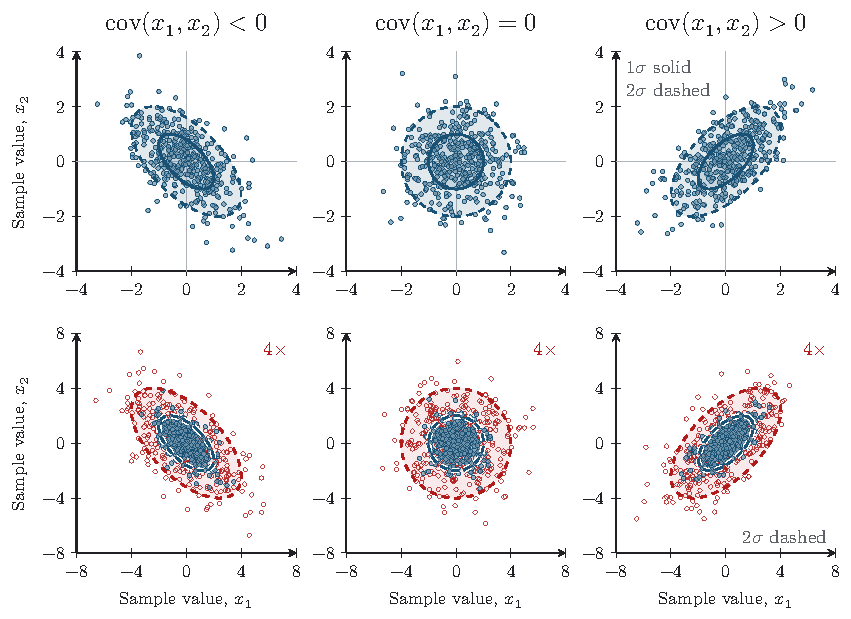
\includegraphics[height=0.81\textheight,keepaspectratio]{../figs/Fig-L5b-Covariance-Schematic.pdf}
  \end{center}
\end{frame}

\begin{frame}{Empirical Covariance Matrix}
  Use $N\ge2$ equally spaced periods of growth-rate data for $M$ firms.
  Align the records so every firm's period $k$ covers the same interval.

  \vspace{0.5em}
  Let $g_k^{(i)}$ be firm $i$'s growth rate in period $k$. Its sample mean is:
  \[
    g'_i=\frac{1}{N}\sum_{k=1}^{N}g_k^{(i)}.
  \]
  The empirical growth-rate covariance matrix
  $\Sg\in\mathbb R^{M\times M}$ has entries:
  \[
    \hat\Sigma_{g,ij}=\frac{1}{N-1}\sum_{k=1}^{N}
      \underbrace{\bigl(g_k^{(i)}-g'_i\bigr)}_{\text{deviation for }i}\;
      \underbrace{\bigl(g_k^{(j)}-g'_j\bigr)}_{\text{deviation for }j},
      \qquad i,j\in\mathcal P.
  \]
  Each entry pairs observations from the same period and has units of year$^{-2}$.
\end{frame}

\begin{frame}{Interpreting the Covariance Matrix}
  The covariance matrix describes individual growth-rate variability and
  how growth rates move together across firms:

  \vspace{0.5em}
  \begin{itemize}\setlength{\itemsep}{0.8em}
    \item \hilite{Diagonal entries}: $\hat\Sigma_{g,ii}$ is firm $i$'s
      growth-rate variance. Its square root is the growth-rate standard
      deviation $\sigma_g$ for that firm (year$^{-1}$).
    \item \hilite{Off-diagonal entries}: positive values mean the two growth
      rates tend to deviate from their means in the same direction;
      negative values mean opposite directions.
  \end{itemize}

  \vspace{0.6em}
  Covariance also depends on the scale of each growth-rate series.
  Next, correlation lets us compare relationships on a common scale.
\end{frame}

\begin{frame}{Correlation}
  For firms $i$ and $j$ with positive sample variances, \hilite{correlation}
  divides growth-rate covariance by the product of their standard deviations:
  \[
    \boxed{\rho_{ij}=\frac{\hat\Sigma_{g,ij}}{\sqrt{\hat\Sigma_{g,ii}\,\hat\Sigma_{g,jj}}}\in[-1,1]
    \quad\Longleftrightarrow\quad
    \hat\Sigma_{g,ij}=\rho_{ij}\sqrt{\hat\Sigma_{g,ii}\,\hat\Sigma_{g,jj}}.}
  \]

  This dimensionless ratio lets us compare pairs of firms:

  \vspace{0.4em}
  \begin{itemize}\setlength{\itemsep}{0.6em}
    \item \hilite{Direction and strength}: the sign gives the direction;
      values closer to $-1$ or $1$ indicate a stronger linear relationship.
    \item \hilite{Zero correlation}: no linear relationship in this sample;
      this does not mean the growth rates are independent.
  \end{itemize}
\end{frame}

\begin{frame}{The Data Matrix and the Sample Covariance}
  Arrange aligned growth rates in $\bG\in\mathbb R^{N\times M}$:
  rows are periods and columns are firms. Compute the covariance matrix
  in two steps:

  \vspace{0.5em}
  \begin{itemize}\setlength{\itemsep}{0.6em}
    \item \hilite{Center each column}: let $\bg'=(g'_1,\ldots,g'_M)^{\top}$
      be the sample-mean vector and $\mathbf 1\in\mathbb R^N$ a vector of ones.
      The outer product repeats these means in every row:
      \[
        \tilde{\bG}=\bG-\mathbf 1\,\bg'^{\top}.
      \]
    \item \hilite{Multiply the centered columns}: the empirical covariance is:
      \[
        \boxed{\Sg=\frac{1}{N-1}\tilde{\bG}^{\top}\tilde{\bG}.}
      \]
  \end{itemize}

  \vspace{0.4em}
  Entry $(i,j)$ is the dot product of centered columns $i$ and $j$, divided
  by $N-1$. This evaluates the earlier covariance formula for every pair at once.
\end{frame}

\begin{frame}{Covariance Matrix Properties}
  The centered-data formula guarantees three properties of our estimate:

  \vspace{0.4em}
  \begin{itemize}\setlength{\itemsep}{0.5em}
    \item \hilite{Elements}: diagonal entries are nonnegative growth-rate
      variances; off-diagonal entries are pairwise covariances.
    \item \hilite{Symmetry}: swapping $i$ and $j$ leaves each product unchanged,
      so $\hat\Sigma_{g,ij}=\hat\Sigma_{g,ji}$.
    \item \hilite{Positive semidefinite}: for any vector $\mathbf v\in\mathbb R^M$,
      the centered-data formula gives:
      \[
        \begin{aligned}
          \mathbf v^{\top}\Sg\mathbf v
          &=\frac{1}{N-1}\mathbf v^{\top}\tilde{\bG}^{\top}\tilde{\bG}\mathbf v\\[0.3em]
          &=\frac{\lVert\tilde{\bG}\mathbf v\rVert_2^2}{N-1}\ge0.
        \end{aligned}
      \]
      This is a squared length divided by $N-1>0$, so every weighted sum
      of growth rates has nonnegative sample variance.
  \end{itemize}

  \vspace{0.4em}
  Scaling by $\Delta t>0$ preserves all three properties.
\end{frame}

\begin{frame}{Estimating the Covariance Rate}
  Under the model, the vector of one-step growth rates $\bg$ has covariance $\Cov(\bg)=\bC/\Delta t$,
  so growth rates and log returns give equivalent estimates of $\bC$:

  \vspace{0.4em}
  \begin{itemize}\setlength{\itemsep}{0.65em}
    \item \hilite{From growth-rate data}: the covariance rate and L4b volatility estimates are:
      \[
        \begin{aligned}
          \Ch&=\Delta t\,\Sg
            &&\text{(year}^{-1}\text{)},\\[0.4em]
          \hat\sigma_i&=\sqrt{\hat C_{ii}}
            =\sqrt{\Delta t}\sqrt{\hat\Sigma_{g,ii}}
            &&\text{(year}^{-1/2}\text{)}.
        \end{aligned}
      \]
    \item \hilite{Comparison with log returns}: $\mathbf r=\Delta t\,\bg$ gives:
      \[
        \hat{\boldsymbol\Sigma}_r=(\Delta t)^2\,\Sg=\Delta t\,\Ch
        \qquad\text{(dimensionless).}
      \]
      For daily data with $\Delta t=1/252$ years, both inputs give:
      \[
        \Ch=\frac{\Sg}{252}=252\,\hat{\boldsymbol\Sigma}_r.
      \]
  \end{itemize}
  These conversions leave correlation unchanged: the common factor cancels.
\end{frame}

\begin{frame}{Example: Covariance and Correlation from Data}
\textbf{\ink{Example:}}
\href{https://github.com/varnerlab/CHEME-5660-CourseRepository-Fall-2026/blob/main/lectures/week-5/L5b/CHEME-5660-L5b-Example-CovarianceMatrix-Fall-2026.ipynb}{Covariance and Correlation from Data}

\vspace{0.8em}
How do firms' growth rates move together?

\vspace{0.6em}
\begin{itemize}\setlength{\itemsep}{0.6em}
  \item Compute the empirical growth-rate covariance matrix and convert it
    to the GBM covariance rate.
  \item Check the covariance calculation and compare the implied volatilities
    with our L4b estimates.
  \item Interpret the covariance and correlation of a pair of firms.
\end{itemize}

\vspace{0.7em}
The estimated covariance tells us how asset growth rates vary together.
Next, we decide how much of our investment to assign to each asset.
\end{frame}

\begin{frame}{Portfolio Weights}
  Once we can simulate several assets together, we need to specify how much
  to invest in each.

  \vspace{0.6em}
  Let $W_0>0$ be initial wealth in dollars, and let
  $\bw=(w_1,\ldots,w_M)^{\top}$ contain the fractions invested at time zero.

  \vspace{0.6em}
  For a fully invested, long-only portfolio, the weights satisfy:
  \[
    \underbrace{w_i\ge0}_{\text{long only}},\qquad
    \underbrace{\sum_{i=1}^{M}w_i=1}_{\text{fully invested}}.
  \]

  \vspace{0.4em}
  These constraints define the $(M-1)$-dimensional \hilite{simplex}
  $\Delta^{M-1}$: a line segment for two assets and a triangle for three.
\end{frame}

\begin{frame}{Buy-and-Hold Wealth}
  We allow fractional shares and ignore dividends and trading costs.
  At time zero, we buy and then hold a fixed number of shares of each asset:
  \[
    n_i=\frac{w_iW_0}{S_i(0)}.
  \]
  Portfolio wealth at time $t$ is:
  \[
    \boxed{W_t=\sum_{i=1}^{M}n_iS_i(t)
      =W_0\sum_{i=1}^{M}w_i\,\frac{S_i(t)}{S_i(0)}.}
  \]

  \vspace{0.4em}
  The fraction of wealth in asset $i$ then becomes:
  \[
    w_i(t)=\frac{n_iS_i(t)}{W_t}.
  \]

  Share counts remain fixed, but weights change as relative prices move.
  Maintaining constant weights requires trading to rebalance the portfolio.
\end{frame}

\begin{frame}{Dirichlet Sampling of the Simplex}
  Draw $\bw\sim\operatorname{Dirichlet}(\boldsymbol\alpha)$, with
  \hilite{concentration parameters} $\boldsymbol\alpha=(\alpha_1,\ldots,\alpha_M)$,
  where $\alpha_i>0$ and $\alpha_0=\sum_{i=1}^{M}\alpha_i$.

  \vspace{0.4em}
  Each draw gives weights that sum to one and are positive with probability one, so the full budget is
  invested. We use a draw as the initial allocation $\bw$. The weight moments are:
  \[
    \begin{gathered}
      \E[w_i]=\frac{\alpha_i}{\alpha_0},\qquad
      \Var(w_i)=\frac{\alpha_i(\alpha_0-\alpha_i)}{\alpha_0^2(\alpha_0+1)},\\[0.5em]
      \Cov(w_i,w_j)=-\frac{\alpha_i\alpha_j}{\alpha_0^2(\alpha_0+1)},\qquad i\ne j.
    \end{gathered}
  \]

  These moments describe the sampled portfolio weights. To evaluate
  portfolio risk, we use the covariance matrix of the firms' growth rates.
\end{frame}

\begin{frame}{How Concentration Shapes the Weights}
  For the three-firm example, changing $\boldsymbol\alpha$ changes how we
  divide the investment:

  \vspace{0.4em}
  \begin{itemize}\setlength{\itemsep}{0.5em}
    \item \hilite{Explore different investment mixes}, $\boldsymbol\alpha=(1,1,1)$:
      no firm is favored; one portfolio might allocate
      70\%, 20\%, and 10\% to the three firms.
    \item \hilite{Concentrate the investment}, $\boldsymbol\alpha=(0.5,0.5,0.5)$:
      favor more uneven allocations, with most money in one or two firms.
    \item \hilite{Stay closer to an equal split}, $\boldsymbol\alpha=(5,5,5)$:
      draws cluster closer to one third of the investment in each firm.
    \item \hilite{Favor the first firm}, $\boldsymbol\alpha=(5,1,1)$:
      it receives about 71\% of the budget on average across draws.
  \end{itemize}

  \vspace{0.5em}
  Both $(1,1,1)$ and $(5,5,5)$ average one third per firm
  \hilite{across many draws}. The larger parameters make
  \hilite{individual portfolios} closer to that equal split.
\end{frame}

\begin{frame}{Linear Portfolio Growth-Rate Proxy}
  How do we compare the portfolios that different allocations produce?
  We summarize each allocation by the mean and variance of its growth rate.

  \vspace{0.5em}
  Hold an allocation $\bw$ for one period of length $\Delta t$, and collect
  the asset growth rates over that period in $\bg=[g_1,\ldots,g_M]^{\top}$.
  Keeping only terms first order in the log returns $g_i\Delta t$:
  \[
    \frac{1}{\Delta t}\ln\!\left(\frac{W_{\Delta t}}{W_0}\right)
    =\frac{1}{\Delta t}\ln\!\left(\sum_{i=1}^{M}w_i e^{g_i\Delta t}\right)
    \approx\bw^{\top}\bg=g_p.
  \]
  We call $g_p$ the \hilite{linear growth-rate proxy}.

  \slidenote{Where is this coming from?}{use $e^{g_i\Delta t}\approx1+g_i\Delta t$,
  then $\sum_iw_i=1$, and then $\ln(1+x)\approx x$.}
\end{frame}

\begin{frame}{Estimating Portfolio Growth and Risk}
  Over the historical observations, the proxy's sample mean and variance are:
  \[
    \begin{aligned}
      g^{\prime}_p&=\bw^{\top}\bg^{\prime}, &&\text{(mean growth rate)}\\[0.4em]
      \sigma_{g,p}^2&=\bw^{\top}\Sg\bw\ge0. &&\text{(variance)}
    \end{aligned}
  \]
  Here, $\bg^{\prime}$ (year$^{-1}$) and $\Sg$ (year$^{-2}$) come from the
  covariance estimate. The variance includes each firm's variability and the
  covariances between firms.

  \vspace{0.6em}
  The proxy covers one period. Over time, we use the wealth formula.
\end{frame}

\begin{frame}{From Sampling to Portfolio Choice}
  A Dirichlet draw gives a candidate allocation. We evaluate its estimated
  growth and risk before choosing how to invest:

  \vspace{0.5em}
  \begin{itemize}\setlength{\itemsep}{0.7em}
    \item \hilite{Sampling}: compare many candidate allocations. The
      lowest-variance draw need not minimize variance over all feasible weights.
    \item \hilite{Optimization in L6a}: solve for weights that minimize
      estimated variance, with or without a required mean growth rate.
  \end{itemize}

  \vspace{0.8em}
  \textbf{\ink{Example:}}
  \href{https://github.com/varnerlab/CHEME-5660-CourseRepository-Fall-2026/blob/main/lectures/week-5/L5b/CHEME-5660-L5b-Example-Dirichlet-PortfolioWeights-Fall-2026.ipynb}{Portfolio Weights and the Dirichlet Distribution}

  Explore investment mixes, compare their estimated growth and risk, and
  follow selected buy-and-hold portfolios using the wealth formula.
\end{frame}

% ==== optional advanced material =============================
\begin{frame}{Optional Advanced Material}
  \textbf{\ink{Advanced:}}
  \href{https://github.com/varnerlab/CHEME-5660-CourseRepository-Fall-2026/blob/main/lectures/week-5/L5b/advanced/ito-derivation/CHEME-5660-L5b-Derivation-MAGBM-Solution-Fall-2026.ipynb}{Derivation of the Multiple Asset GBM Solution}

  Why does each asset's drift correction contain only its own variance rate?
  We extend It\^o's lemma to several noise sources and derive the scaling rule.

  \vspace{0.8em}
  \textbf{\ink{Advanced:}}
  \href{https://github.com/varnerlab/CHEME-5660-CourseRepository-Fall-2026/blob/main/lectures/week-5/L5b/advanced/covariance-estimation/CHEME-5660-L5b-Advanced-CovarianceEstimation-Fall-2026.ipynb}{Sampling Error and Covariance Shrinkage}

  How does estimation error affect portfolio selection? We measure covariance
  error, combine the sample estimate with a simpler matrix, and compare the
  resulting minimum-variance portfolios on later data.

  \vspace{0.8em}
  \textbf{\ink{Advanced:}}
  \href{https://github.com/varnerlab/CHEME-5660-CourseRepository-Fall-2026/blob/main/lectures/week-5/L5b/advanced/rolling-correlation/CHEME-5660-L5b-Advanced-RollingCorrelation-Fall-2026.ipynb}{Rolling Correlations}

  Are the relationships between firms stable over time? We compare rolling and
  exponentially weighted correlations and examine changes during periods of
  high market volatility.

  \vspace{0.6em}
  \dimmed{Optional; none of these notebooks is a prerequisite for L6a.}
\end{frame}

\begin{frame}{Summary}
  We modeled correlated asset prices and examined how the fraction invested
  in each firm affected portfolio growth and risk.

  \vspace{0.5em}
  {\large\textbf{\ink{Key takeaways}}}
  \vspace{0.3em}
  \begin{itemize}\setlength{\itemsep}{0.4em}
    \item \hilite{Correlated asset prices}: We reviewed EMA parameter updates,
      then combined independent Wiener increments with a loading matrix to model firms whose prices move together.
    \item \hilite{Covariance from data}: We estimated growth-rate covariance,
      scaled it by the observation interval to obtain the covariance rate,
      and used correlation to compare co-movement across firms.
    \item \hilite{Portfolio weights}: We used Dirichlet draws to explore
      investment mixes, compared them with a linear growth-rate proxy, and
      calculated buy-and-hold wealth from fixed share counts.
  \end{itemize}
\end{frame}

\transitionframe{Next time: we will use minimum-variance optimization to find
optimal portfolio weights---the weights that minimize estimated variance
under the chosen constraints.}

\end{document}
